\chapter{Batterijen, brandstofcellen en elektrolyse}\label{ch:b2:batteries-electrolysis}

Elke kilogram aluminium die uit zijn erts gewonnen wordt, kost ongeveer \qty{13}{kW.h}
elektriciteit; een kilogram schroot omsmelten kost in principe de
\qty{0.3}{kW.h} die het tot zijn smeltpunt opwarmt en het doet smelten. Het verschil
is het werk van een lange rij elektrolysecellen, die elk honderdduizenden
ampère door gesmolten zout sturen bij een paar volt. Een batterij werkt
in de andere richting: een spontane reactie drijft de stroom aan. Met de
\omterm{def:b2:current-potential-curves:ie-curve}{stroom-potentiaalkrommen} van \cref{ch:b2:current-potential-curves} worden beide
in hetzelfde diagram gelezen, net als een stuk zink dat in zuur oplost.
% ledger: hT:Al_l.933, aw:Al

\begin{recall}
\Cref{ch:b2:cell-thermodynamics}: $\Delta_r G = -nFE$, maximale arbeid, de
\omterm{def:b2:cell-thermodynamics:faraday}{constante van Faraday}. \Cref{ch:b2:current-potential-curves}: \omterm{def:b2:current-potential-curves:ie-curve}{stroom-potentiaalkrommen},
snelle en trage systemen, \omterm{def:b2:current-potential-curves:overpotential}{overspanningen}, \omterm{def:b2:current-potential-curves:limiting-current}{grensstromen}, de muren van
water. \Cref{ch:b2:ellingham}: waarom aluminium niet met koolstof gewonnen wordt. Het
schoolboek: \omterm{def:b2:batteries-electrolysis:electrolysis}{elektrolyse}, \omterm{def:b2:batteries-electrolysis:battery}{accumulatoren}.
\end{recall}

\begin{omfigure}
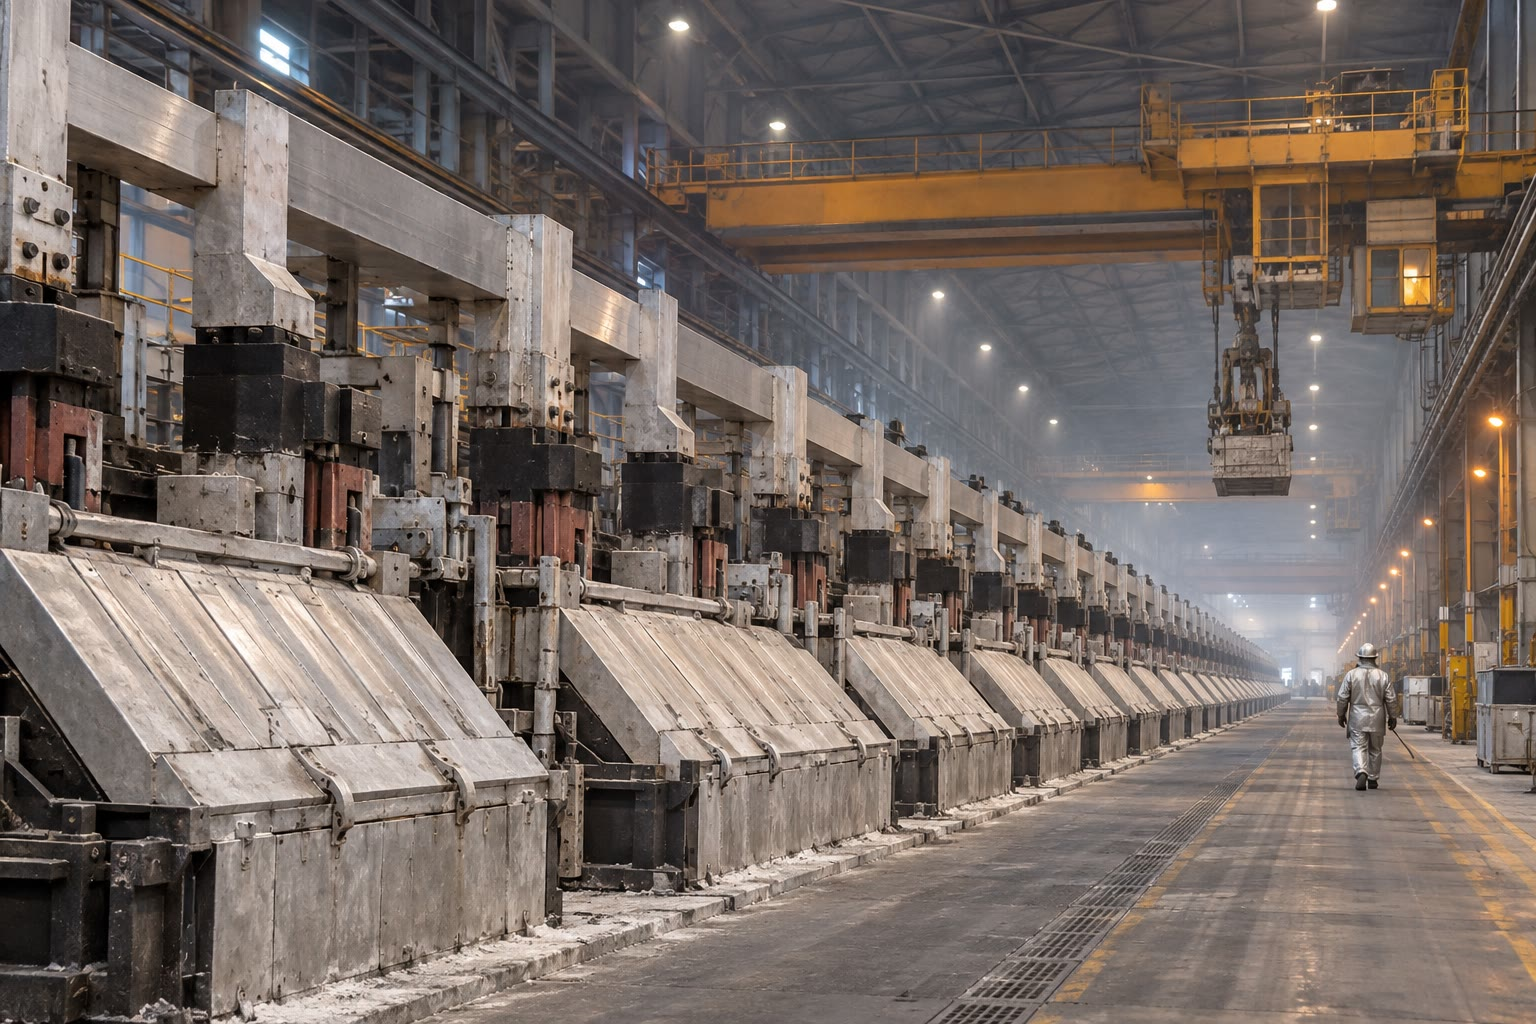
\includegraphics[width=0.62\linewidth]{images/book3/ai/b2-11-potroom.jpg}

{\small De elektrolysehal van een aluminiumsmelterij: een rij elektrolysecellen,
honderden lang, in serie geschakeld; de loopkraan vervangt de koolstofanoden
naarmate ze opbranden.}
\end{omfigure}

\section{Spontane reacties gelezen op krommen}

\begin{definition}[Gemengde potentiaal]\label{def:b2:batteries-electrolysis:mixed-potential}
De \emph{gemengde potentiaal}\index{gemengde potentiaal} van een elektrode waarop twee
verschillende koppels reageren, het ene geoxideerd en het andere gereduceerd, is de potentiaal die ze
aanneemt wanneer er geen netto stroom loopt: de \omterm{def:b2:current-potential-curves:ie-curve}{anodische stroom} van het ene koppel is dan
even groot als en tegengesteld aan de \omterm{def:b2:current-potential-curves:ie-curve}{kathodische stroom} van het andere.
\end{definition}

\begin{proposition}[Een metaal in een oplossing]\label{prop:b2:batteries-electrolysis:mixed}
Een metaal dat ondergedompeld is in een oplossing die het kan oxideren, neemt de potentiaal
$E_m$ aan waarbij $i_a(E_m) = -i_c(E_m)$: de \omterm{def:b2:current-potential-curves:ie-curve}{anodische stroom} van de oxidatie van het
metaal compenseert de \omterm{def:b2:current-potential-curves:ie-curve}{kathodische stroom} van de reductie van de oxidator; het
metaal lost op met de snelheid $i_a(E_m)/(nF)$.
\end{proposition}

\begin{proof}
Een geïsoleerd stuk metaal voert geen netto stroom. Beide halfreacties verlopen
aan zijn oppervlak bij dezelfde potentiaal, dus hun stromen, afgelezen op hun krommen
bij die potentiaal, zijn samen nul. Volgens \cref{prop:b2:current-potential-curves:current-rate}
geeft de \omterm{def:b2:current-potential-curves:ie-curve}{anodische stroom} de oxidatiesnelheid.
\end{proof}

\begin{omfigure}
\begin{tikzpicture}
\begin{axis}[omie, width=0.82\linewidth, height=6cm, xmin=-1.1, xmax=-0.3,
  ymin=-3, ymax=3, xlabel={$E$ (V)}, ylabel={$i$}, clip=true, clip mode=individual,
  axis y line=left]
\addplot[omanodic] table[x=E, y=i] {figdata/out/bachelor-2-ie-curves-f-Zn.dat};
\addplot[omcathodic] table[x=E, y=i] {figdata/out/bachelor-2-ie-curves-f-HZn.dat};
\addplot[omcathodic, dashed] table[x=E, y=i] {figdata/out/bachelor-2-ie-curves-f-HCu.dat};
\draw[densely dotted] (axis cs:-0.820,-0.148) -- (axis cs:-0.820,0.148);
\draw[densely dotted] (axis cs:-0.737,-2.38) -- (axis cs:-0.737,2.38);
\fill (axis cs:-0.820,0.148) circle (1.3pt); \fill (axis cs:-0.737,2.38) circle (1.3pt);
\node[font=\scriptsize, anchor=south east] at (axis cs:-0.825,0.2) {zink alleen};
\node[font=\scriptsize, anchor=west] at (axis cs:-0.73,2.38) {zink in contact met koper};
\node[font=\scriptsize, omThm, anchor=west] at (axis cs:-0.70,1.2) {\ce{Zn} $\to$ \ce{Zn^2+}};
\node[font=\scriptsize, omDef, anchor=north west, align=left] at (axis cs:-0.87,-0.5) {\ce{H+} $\to$ \ce{H2}\\ op zink};
\node[font=\scriptsize, omDef, anchor=north west] at (axis cs:-0.66,-1.7) {op koper};
\end{axis}
\end{tikzpicture}

{\small Zink in zuur (modelkrommen, zinkionen verdund; potentialen van
$-1.1$ tot \qty{-0.3}{V}). Op zichzelf neemt zink
de \omterm{def:b2:batteries-electrolysis:mixed-potential}{gemengde potentiaal} aan waarbij zijn oxidatie de trage reductie van
\ce{H+} op zink compenseert: een kleine stroom, een traag oplossen. In contact met koper, waarop
de reductie van \ce{H+} minder traag is, verschuift het evenwicht naar een hogere potentiaal
en een meer dan tien keer grotere stroom: het zink lost snel op, en waterstof
borrelt op het koper.}
\end{omfigure}

Dezelfde lezing verklaart corrosie (\cref{ch:b2:corrosion}): de corrosiesnelheid
van een metaal is de stroom bij zijn \omterm{def:b2:batteries-electrolysis:mixed-potential}{gemengde potentiaal}.

\section{Cellen die een stroom leveren}

\begin{definition}[Batterijen]\label{def:b2:batteries-electrolysis:battery}
Een \emph{primaire cel}\index{primaire cel} is een elektrochemische cel die
één keer gebruikt wordt, tot haar reagentia op zijn. Een \emph{accumulator}\index{accumulator}
is een cel die opnieuw geladen kan worden door er een stroom in de
omgekeerde richting door te sturen, wat haar reactie omkeert. De \emph{specifieke
energie}\index{specifieke energie} van een cel is de elektrische energie die ze levert
per eenheid massa, meestal in \unit{W.h/kg}.
\end{definition}

\begin{proposition}[Spanning van een cel die een stroom levert]\label{prop:b2:batteries-electrolysis:delivering}
Een cel die een stroom $I$ levert, heeft een spanning
\[
  U = E_+ - E_- - \eta_a - |\eta_c| - rI ,
\]
waarin $E_+$ en $E_-$ de evenwichtspotentialen van haar twee elektroden zijn,
$\eta_a > 0$ de \omterm{def:b2:current-potential-curves:overpotential}{overspanning} van de oxidatie aan de negatieve elektrode,
$\eta_c < 0$ die van de reductie aan de positieve elektrode, en $r$ de
inwendige weerstand (elektrolyt, scheider, verbindingen).
\end{proposition}

\begin{proof}
Dezelfde stroom $I$ is anodisch aan de negatieve elektrode, waarvan de potentiaal
afgelezen wordt op haar anodische kromme, $E_- + \eta_a$, en kathodisch aan de positieve,
waarvan de potentiaal $E_+ + \eta_c$ is. Daartussen steekt de stroom het
elektrolyt over, waar de potentiaal met $rI$ daalt. Dus $U = (E_+ + \eta_c) - (E_- +
\eta_a) - rI$.
\end{proof}

\begin{omfigure}
\begin{tikzpicture}
\begin{axis}[omie, width=0.82\linewidth, height=5.6cm, xmin=-1.2, xmax=0.8,
  ymin=-2, ymax=2, xlabel={$E$ (V)}, ylabel={$i$}, clip=true, clip mode=individual]
\addplot[omanodic] table[x=E, y=i] {figdata/out/bachelor-2-ie-curves-h-neg.dat};
\addplot[omcathodic] table[x=E, y=i] {figdata/out/bachelor-2-ie-curves-h-pos.dat};
\draw[densely dashed, gray] (axis cs:-1.2,1) -- (axis cs:0.8,1);
\draw[densely dashed, gray] (axis cs:-1.2,-1) -- (axis cs:0.8,-1);
\node[font=\scriptsize, gray, anchor=south west] at (axis cs:-1.18,1) {$+I$};
\node[font=\scriptsize, gray, anchor=north west] at (axis cs:-1.18,-1) {$-I$};
\fill (axis cs:-0.730,1) circle (1.3pt); \fill (axis cs:0.210,-1) circle (1.3pt);
\draw[densely dotted] (axis cs:-0.85,0) -- (axis cs:-0.85,0.5);
\draw[densely dotted] (axis cs:0.45,0) -- (axis cs:0.45,-0.5);
\node[font=\scriptsize, anchor=south] at (axis cs:-0.85,0.5) {$E_-$};
\node[font=\scriptsize, anchor=north] at (axis cs:0.45,-0.5) {$E_+$};
\draw[<->, thick, omProp] (axis cs:-0.730,1.5) -- (axis cs:0.210,1.5) node[midway, above, font=\scriptsize] {$U + rI$};
\draw[densely dotted] (axis cs:-0.730,1) -- (axis cs:-0.730,1.5);
\draw[densely dotted] (axis cs:0.210,-1) -- (axis cs:0.210,1.5);
\node[font=\scriptsize, omThm, anchor=west] at (axis cs:-0.70,0.6) {negatieve elektrode};
\node[font=\scriptsize, omDef, anchor=west] at (axis cs:0.30,-1.5) {positieve elektrode};
\end{axis}
\end{tikzpicture}

{\small Het werkpunt van een cel (modelkrommen). Bij een stroom $I$ zit de
negatieve elektrode op haar anodische kromme, de positieve elektrode op haar
kathodische kromme; het verschil van de twee potentialen, verminderd met de ohmse val
$rI$, is de geleverde spanning. Die daalt naarmate $I$ groeit.}
\end{omfigure}

\begin{method}[Het werkpunt van een cel of een elektrolysecel]\label{met:b2:batteries-electrolysis:operating-point}
\begin{enumerate}
  \item Teken de anodische kromme van de elektrode die geoxideerd wordt en de
        kathodische kromme van die welke gereduceerd wordt.
  \item Lees voor een stroom $I$ de potentiaal van elke elektrode af bij $+I$ op de
        anodische kromme en bij $-I$ op de kathodische.
  \item Het verschil van de twee potentialen, gecorrigeerd met $rI$ (afgetrokken voor
        een cel, opgeteld voor een \omterm{def:b2:batteries-electrolysis:electrolysis}{elektrolysecel}), is de spanning.
\end{enumerate}
\end{method}

\begin{example}[De loodaccumulator]\label{ex:b2:batteries-electrolysis:lead}
Aan de negatieve elektrode \ce{Pb + SO4^2- -> PbSO4 + 2e-}; aan de positieve
\ce{PbO2 + 4H+ + SO4^2- + 2e- -> PbSO4 + 2H2O}. In totaal
\[
  \ce{Pb + PbO2 + 4H+ + 2SO4^2- -> 2PbSO4 + 2H2O},
\]
$\Delta_r G^\circ = 2(-813.14) + 2(-237.13) - (-217.33) - 2(-744.53) =
\qty{-394.1}{kJ/mol}$, $E^\circ = 394\,100/(2 \times 96\,485) = \qty{2.04}{V}$.
Beide elektroden raken bedekt met loodsulfaat terwijl de cel ontlaadt; laden
keert de reactie om. De reductie van \ce{H+} op lood en de oxidatie van
water op looddioxide zijn traag: daarom kan een cel van \qty{2}{V} geladen worden
in water, waarvan het thermodynamische venster slechts \qty{1.23}{V} breed is.
% ledger: dfg:PbSO4_cr, dfg:H2O_l, dfg:PbO2_cr, dfg:SO42-_ao
\end{example}

\begin{omfigure}
\begin{tikzpicture}[font=\small, >={Stealth}]
  \draw[thick] (0,0) rectangle (6,3.2);
  \fill[omDef!10] (0.05,0.05) rectangle (5.95,2.7);
  \fill[black!45] (0.6,0.4) rectangle (1.1,2.9);
  \fill[brown!60!black] (4.9,0.4) rectangle (5.4,2.9);
  \draw[thick] (0.85,2.9) -- (0.85,3.9) node[pos=0.75, left] {$-$};
  \draw[thick] (5.15,2.9) -- (5.15,3.9) node[pos=0.75, right] {$+$};
  \draw[->, thick, omProp] (0.85,3.9) -- (0.85,4.3) -- (5.15,4.3) -- (5.15,3.95);
  \node[font=\scriptsize, omProp, anchor=south] at (3,4.3) {$\mathrm{e^-}$ bij ontladen};
  \node[font=\scriptsize, align=center] at (0.85,-0.45) {\ce{Pb}\\ (\ce{PbSO4} bij ontladen)};
  \node[font=\scriptsize, align=center] at (5.15,-0.45) {\ce{PbO2}\\ (\ce{PbSO4} bij ontladen)};
  \node[font=\scriptsize, align=center] at (3.0,1.6) {oplossing \ce{H2SO4}\\ \ce{H+}, \ce{HSO4-}, \ce{SO4^2-}};
\end{tikzpicture}

{\small De loodaccumulator, schematisch. Bij het ontladen wordt lood geoxideerd
en looddioxide gereduceerd, beide tot loodsulfaat, en wordt het zuur verbruikt: de
dichtheid van de oplossing geeft de laadtoestand aan.}
\end{omfigure}

\begin{omfigure}
\begin{tikzpicture}[font=\small, >={Stealth}]
  \draw[thick] (0,0) rectangle (7,3);
  % graphite layers
  \foreach \y in {0.5,0.9,1.3,1.7,2.1,2.5} \draw[thick, black!70] (0.3,\y) -- (2.3,\y);
  \foreach \y in {0.7,1.1,1.5,1.9,2.3} \foreach \x in {0.6,1.3,2.0} \fill[omDef] (\x,\y) circle (0.07);
  % layered oxide
  \foreach \y in {0.5,0.9,1.3,1.7,2.1,2.5} \draw[thick, omThm] (4.7,\y) -- (6.7,\y);
  \foreach \y in {0.7,1.5,2.3} \foreach \x in {5.0,5.7,6.4} \fill[omDef] (\x,\y) circle (0.07);
  \draw[densely dashed] (3.5,0) -- (3.5,3);
  \node[font=\scriptsize, align=center] at (1.3,-0.45) {grafiet (negatief)};
  \node[font=\scriptsize, align=center] at (5.7,-0.45) {gelaagd oxide (positief)};
  \node[font=\scriptsize, anchor=south] at (3.5,3.0) {scheider};
  \draw[->, thick, omThm] (2.5,2.1) -- (4.5,2.1) node[midway, above, font=\scriptsize, fill=white, inner sep=1pt] {\ce{Li+} bij ontladen};
  \draw[<-, thick, omDef] (2.5,0.9) -- (4.5,0.9) node[midway, below, font=\scriptsize, fill=white, inner sep=1pt] {\ce{Li+} bij laden};
\end{tikzpicture}

{\small Een lithium-ioncel, schematisch. Lithiumionen (blauwe stippen) zitten tussen de
lagen van het grafiet in de geladen cel; bij het ontladen steken ze het
elektrolyt over en schuiven ze tussen de lagen van een metaaloxide, terwijl de elektronen
via de uitwendige keten gaan. Geen van beide elektroden wordt opgelost of afgezet: de
ionen pendelen tussen twee gastheren.}
\end{omfigure}

\begin{history}[De zuil van Volta]
\begin{minipage}[t]{0.27\linewidth}
\vspace{0pt}
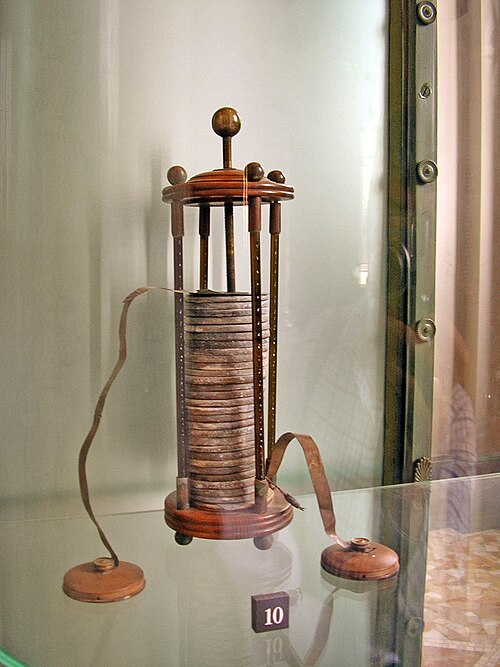
\includegraphics[width=\linewidth]{images/book3/volta-pile.jpg}
\end{minipage}\hfill
\begin{minipage}[t]{0.69\linewidth}
\vspace{0pt}
In 1800 beschreef Alessandro Volta een zuil van schijven van twee verschillende metalen,
zink en koper of zilver, gescheiden door in pekel gedrenkte doek: de eerste
bron van een constante elektrische stroom. Binnen enkele weken gebruikten anderen haar om
water te ontleden, en binnen tien jaar had Humphry Davy natrium en kalium geïsoleerd door
\omterm{def:b2:batteries-electrolysis:electrolysis}{elektrolyse} van hun gesmolten hydroxiden met een grote zuil. De foto toont
een van Volta's eigen zuilen. (Foto: GuidoB, CC BY-SA 3.0, Wikimedia
Commons.)
\end{minipage}
\end{history}

\section{Brandstofcellen}

\begin{definition}[Brandstofcel]\label{def:b2:batteries-electrolysis:fuel-cell}
Een \emph{brandstofcel}\index{brandstofcel} is een cel waarvan de reagentia, een brandstof en een
oxidator (meestal de zuurstof van de lucht), continu naar haar elektroden
gevoerd worden en waarvan de producten verwijderd worden, zodat ze stroom levert zolang
ze gevoed wordt.
\end{definition}

In de cel met protonwisselend membraan van de bus van
\cref{ch:b2:cell-thermodynamics} wordt waterstof geoxideerd op een platinakatalysator,
\ce{H2 -> 2H+ + 2e-}, steken protonen een dun, zuur polymeermembraan over, en wordt zuurstof
aan de andere kant gereduceerd, \ce{O2 + 4H+ + 4e- -> 2H2O}. De oxidatie van waterstof
op platina is een \omterm{def:b2:current-potential-curves:fast-slow}{snel systeem}; de reductie van zuurstof is traag op elke
elektrode. Het grootste deel van het spanningsverlies tussen de \qty{1.23}{V} van de reversibele
cel en de werkspanning is de \omterm{def:b2:current-potential-curves:overpotential}{overspanning} van de zuurstofelektrode,
de rest de weerstand van het membraan en, bij hoge stroom, de aanvoer van
zuurstof naar de katalysator (een \omterm{def:b2:current-potential-curves:limiting-current}{grensstroom}).

\section{Elektrolyse}

\begin{definition}[Elektrolyse]\label{def:b2:batteries-electrolysis:electrolysis}
Een \emph{elektrolyse}\index{elektrolyse} is een niet-spontane redoxreactie
die afgedwongen wordt door een stroom van een uitwendige generator; de cel waarin ze
plaatsvindt, is een \emph{elektrolysecel}\index{elektrolysecel}. De anode, waar de
oxidatie plaatsvindt, is verbonden met de positieve pool van de generator.
\end{definition}

\begin{proposition}[Thermodynamische minimumspanning]\label{prop:b2:batteries-electrolysis:minimum-voltage}
Een \omterm{def:b2:batteries-electrolysis:electrolysis}{elektrolyse} waarvan de reactie $\Delta_r G > 0$ heeft, vereist een spanning van ten
minste $\Delta_r G/(nF)$.
\end{proposition}

\begin{proof}
De generator levert de arbeid $nFU$ per mol reactie; volgens
\cref{thm:b2:cell-thermodynamics:delta-g-nfe}, toegepast op de omgekeerde reactie, moet de
ontvangen elektrische arbeid ten minste $\Delta_r G$ zijn.
\end{proof}

\begin{proposition}[Spanning van een elektrolysecel]\label{prop:b2:batteries-electrolysis:electrolysis-voltage}
Een \omterm{def:b2:batteries-electrolysis:electrolysis}{elektrolysecel} waardoor een stroom $I$ loopt, heeft nodig
\[
  U = (E_a - E_c) + \eta_a + |\eta_c| + rI ,
\]
met $E_a$, $E_c$ de evenwichtspotentialen van het anode- en het kathodekoppel
($E_a - E_c = \Delta_r G/(nF)$), $\eta_a$, $\eta_c$ hun \omterm{def:b2:current-potential-curves:overpotential}{overspanningen} bij die
stroom en $r$ de weerstand tussen de elektroden.
\end{proposition}

\begin{proof}
Zoals voor een cel is dezelfde stroom anodisch aan de anode, bij potentiaal $E_a +
\eta_a$, en kathodisch aan de kathode, bij $E_c + \eta_c$; de generator moet hem bovendien
door het elektrolyt drijven, wat $rI$ toevoegt.
\end{proof}

\begin{method}[Een elektrolyse voorspellen]\label{met:b2:batteries-electrolysis:predict-electrolysis}
\begin{enumerate}
  \item Som elk deeltje op dat aan de anode geoxideerd kan worden (het
        anodemetaal en het oplosmiddel inbegrepen) en elk deeltje dat aan
        de kathode gereduceerd kan worden (het oplosmiddel inbegrepen).
  \item Teken hun \omterm{def:b2:current-potential-curves:ie-curve}{stroom-potentiaalkrommen} op de gebruikte elektrodematerialen.
  \item Naarmate de spanning stijgt, geven de eerste anodische kromme en de eerste kathodische
        kromme die bereikt worden de reacties; bij grotere stromen voegen de volgende
        de hunne toe.
\end{enumerate}
\end{method}

\begin{definition}[Stroomrendement]\label{def:b2:batteries-electrolysis:faradaic-efficiency}
Het \emph{stroomrendement}\index{stroomrendement} $\eta_F$ van een
\omterm{def:b2:batteries-electrolysis:electrolysis}{elektrolyse} is de fractie van de doorgevoerde lading die het gewenste
product oplevert. Het \emph{specifiek energieverbruik}\index{specifiek energieverbruik}
is de elektrische energie die per eenheid massa product verbruikt wordt.
\end{definition}

\begin{proposition}[Wet van Faraday]\label{prop:b2:batteries-electrolysis:faraday-mass}
Een stroom $I$ die gedurende een tijd $t$ wordt doorgevoerd met \omterm{def:b2:batteries-electrolysis:faradaic-efficiency}{stroomrendement} $\eta_F$, levert een
massa $m = \eta_F MIt/(nF)$ van een product met molaire massa $M$ dat gevormd wordt met $n$
elektronen per mol.
\end{proposition}

\begin{proof}
De lading $It$, waarvan $\eta_F It$ het product vormt, komt volgens
\cref{prop:b2:cell-thermodynamics:charge} overeen met $\eta_F It/(nF)$ mol.
\end{proof}

\begin{proposition}[Energie per kilogram]\label{prop:b2:batteries-electrolysis:energy}
Bij een spanning $U$ en \omterm{def:b2:batteries-electrolysis:faradaic-efficiency}{stroomrendement} $\eta_F$ is het \omterm{def:b2:batteries-electrolysis:faradaic-efficiency}{specifiek
energieverbruik} $w = nFU/(\eta_F M)$.
\end{proposition}

\begin{proof}
De energie is $UIt$ en de massa $\eta_F MIt/(nF)$; deel op elkaar.
\end{proof}

\section{Industriële elektrolyses}

\paragraph{Zink.} Het meeste zink wordt gewonnen door \omterm{def:b2:batteries-electrolysis:electrolysis}{elektrolyse} van de zure
zinksulfaatoplossing van \cref{ch:b2:ellingham}. Zink zet zich af op de kathode hoewel
\ce{H+} de sterkere oxidator is: op zink is de reductie van \ce{H+} zeer traag,
en de zinkgolf wordt eerst bereikt; de anode geeft zuurstof af.

\begin{omfigure}
\begin{tikzpicture}
\begin{axis}[omie, width=0.82\linewidth, height=5.6cm, xmin=-1.6, xmax=2.4,
  ymin=-2.4, ymax=2.4, xlabel={$E$ (V)}, ylabel={$i$}, clip=true, clip mode=individual]
\addplot[omcathodic] table[x=E, y=i] {figdata/out/bachelor-2-ie-curves-g-cath.dat};
\addplot[omanodic] table[x=E, y=i] {figdata/out/bachelor-2-ie-curves-g-an.dat};
\draw[densely dotted] (axis cs:-0.76,-2.2) -- (axis cs:-0.76,0.4);
\draw[densely dotted] (axis cs:0,-2.2) -- (axis cs:0,0.4);
\node[font=\scriptsize, anchor=south] at (axis cs:-0.76,0.4) {$-0.76$};
\node[font=\scriptsize, anchor=south east] at (axis cs:-0.02,0.4) {$0$};
\node[font=\scriptsize, omDef, anchor=north west, align=left] at (axis cs:-0.7,-1.05) {\ce{Zn^2+} $\to$ \ce{Zn},\\ plateau};
\node[font=\scriptsize, omDef, anchor=east, align=right] at (axis cs:-1.32,-0.9) {\ce{H+} $\to$ \ce{H2}\\ op Zn};
\node[font=\scriptsize, omThm, anchor=east] at (axis cs:1.85,1.6) {\ce{H2O} $\to$ \ce{O2}};
\node[font=\scriptsize, gray, align=center] at (axis cs:-0.38,-0.5) {hier geen \ce{H2}\\ op zink};
\end{axis}
\end{tikzpicture}

{\small \omterm{def:b2:batteries-electrolysis:electrolysis}{Elektrolyse} van een zure zinksulfaatoplossing met een zinkkathode
(modelkrommen). Hoewel het koppel \ce{H+}/\ce{H2} ($\qty{0}{V}$) boven
\ce{Zn^2+}/\ce{Zn} ($\qty{-0.76}{V}$) ligt, begint de reductie van \ce{H+} op zink
niet vóór ongeveer \qty{-1.1}{V}: daartussen zet zink zich alleen af. Aan de
anode wordt water tot zuurstof geoxideerd.}
\end{omfigure}

\paragraph{Chloor en natriumhydroxide.} Pekel wordt geëlektrolyseerd in een cel
die gedeeld is door een membraan dat alleen kationen doorlaat. Aan de anode wordt chloride
geoxideerd, \ce{2Cl- -> Cl2 + 2e-}; aan de kathode wordt water gereduceerd, \ce{2H2O +
2e- -> H2 + 2OH-}; natriumionen steken het membraan over om de lading te compenseren, en een
natriumhydroxide-oplossing verlaat de kathodekant, vrij van chloride. Het
thermodynamische minimum is $\Delta_r G/(2F) = \qty{2.19}{V}$ voor \ce{2Cl- + 2H2O -> Cl2 +
H2 + 2OH-} onder standaardomstandigheden. Aan de anode ontstaat chloor in plaats van
zuurstof, hoewel het koppel \ce{O2}/\ce{H2O} lager ligt: de oxidatie van water
is van de twee de traagste op de gebruikte anodematerialen.
% ledger: dfg:OH-_ao, dfg:Cl-_ao, dfg:H2O_l

\begin{omfigure}
\begin{tikzpicture}[font=\small, >={Stealth}]
  \draw[thick] (0,0) rectangle (6,3.4);
  \draw[thick, dashed, omProp] (3,0) -- (3,3.4);
  \fill[black!30] (0.4,0.3) rectangle (0.7,3.0);
  \fill[black!50] (5.3,0.3) rectangle (5.6,3.0);
  \node[font=\scriptsize] at (0.55,3.3) {$+$};
  \node[font=\scriptsize] at (5.45,3.3) {$-$};
  \node[font=\scriptsize, align=center] at (1.85,1.9) {pekel\\ \ce{2Cl-} $\to$\\ \ce{Cl2 + 2e-}};
  \node[font=\scriptsize, align=center] at (4.2,1.9) {\ce{NaOH}-\\ oplossing\\ \ce{2H2O + 2e-} $\to$\\ \ce{H2 + 2OH-}};
  \draw[->, thick, omDef] (2.6,0.8) -- (3.4,0.8) node[pos=0.1, above, font=\scriptsize] {\ce{Na+}};
  \draw[->, thick] (1.0,3.4) -- (1.0,4.0) node[above] {\ce{Cl2}};
  \draw[->, thick] (5.0,3.4) -- (5.0,4.0) node[above] {\ce{H2}};
  \draw[->, thick] (-0.8,0.6) -- (0,0.6) node[pos=0, left] {pekel in};
  \draw[->, thick] (6,0.6) -- (6.8,0.6) node[right] {\ce{NaOH} uit};
  \node[font=\scriptsize, omProp, anchor=north] at (3,-0.05) {kationwisselend membraan};
\end{tikzpicture}

{\small Een membraancel voor chloor en loog, schematisch. Alleen natriumionen steken het
membraan over, zodat het hydroxide dat aan de kathode ontstaat het chloor niet ontmoet.}
\end{omfigure}

\paragraph{Aluminium.} Aluminiumoxide wordt opgelost in gesmolten kryoliet,
\ce{Na3AlF6}, dat veel lager smelt dan aluminiumoxide, en geëlektrolyseerd tussen een
koolstofkathode, waarop vloeibaar aluminium zich verzamelt, en koolstofanoden die
opbranden tot koolstofdioxide (proces van Hall--Héroult):
\[
  \ce{2Al2O3 + 3C -> 4Al + 3CO2} .
\]
Het thermodynamische minimum rond \qty{1250}{K} is ongeveer \qty{1.18}{V}
(\cref{pb:b2:batteries-electrolysis:1}); de cel van dat probleem werkt bij drie
en een half keer zoveel, en het overschot wordt omgezet in de warmte die het bad
gesmolten houdt.

\begin{omfigure}
\begin{tikzpicture}[font=\small, >={Stealth}]
  \draw[thick, fill=black!12] (0,0) rectangle (7,3.2);
  \fill[black!45] (0.3,0.3) rectangle (6.7,0.8);
  \fill[gray!35] (0.3,0.8) rectangle (6.7,1.4);
  \fill[orange!30] (0.3,1.4) rectangle (6.7,2.5);
  \foreach \x in {1.0,3.0,5.0} {
    \fill[black!75] (\x,1.75) rectangle (\x+1.0,3.6);
    \draw[thick] (\x+0.5,3.6) -- (\x+0.5,4.2);
  }
  \draw[thick] (1.5,4.2) -- (5.5,4.2) node[right] {$+$};
  \node[font=\scriptsize, align=left, anchor=west] at (7.3,2.6) {koolstofanoden, verbrand tot \ce{CO2}};
  \node[font=\scriptsize, align=left, anchor=west] at (7.3,1.95) {gesmolten kryoliet + opgelost \ce{Al2O3}};
  \node[font=\scriptsize, align=left, anchor=west] at (7.3,1.1) {vloeibaar aluminium (kathode)};
  \node[font=\scriptsize, align=left, anchor=west] at (7.3,0.55) {koolstofkathodeblok, $-$};
  \draw[densely dotted] (6.7,2.6) -- (7.3,2.6) (6.7,1.95) -- (7.3,1.95) (6.7,1.1) -- (7.3,1.1) (6.7,0.55) -- (7.3,0.55);
\end{tikzpicture}

{\small Een cel van Hall--Héroult, doorsnede, schematisch. Aluminium wordt gereduceerd
aan het oppervlak van het vloeibare metaalbad, dat als kathode werkt; de oxide-ionen
ontladen op de koolstofanoden, die ze tot koolstofdioxide verbranden.}
\end{omfigure}

\begin{history}[Hall en Héroult, 1886]
\begin{minipage}[t]{0.18\linewidth}
\vspace{0pt}
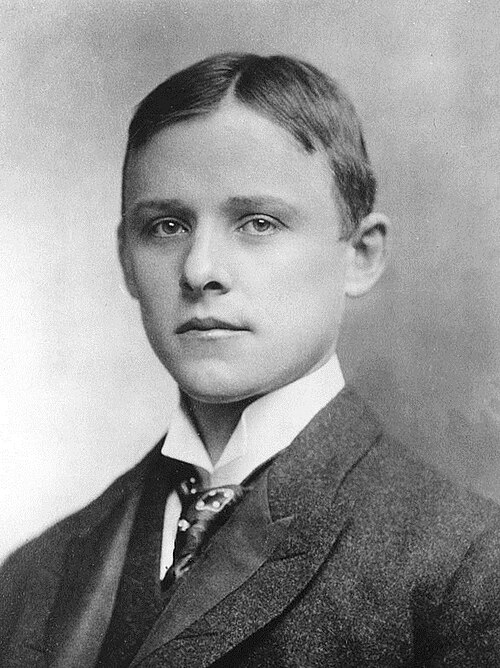
\includegraphics[width=\linewidth]{images/book3/hall.jpg}
\end{minipage}\hspace{0.02\linewidth}%
\begin{minipage}[t]{0.18\linewidth}
\vspace{0pt}
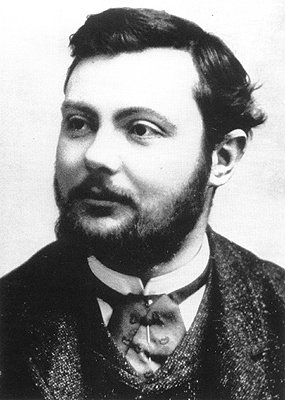
\includegraphics[width=\linewidth]{images/book3/heroult.jpg}
\end{minipage}\hfill
\begin{minipage}[t]{0.58\linewidth}
\vspace{0pt}
In 1886, op hun tweeëntwintigste of drieëntwintigste, ontdekten Charles Martin Hall en
Paul Héroult, aan de twee kanten van de Atlantische Oceaan, onafhankelijk van elkaar dat aluminiumoxide
oplost in gesmolten kryoliet en daar geëlektrolyseerd kan worden. Aluminium, tot
dan toe een edelmetaal dat gemaakt werd door zijn chloride met natrium te reduceren, werd het
goedkoopste van de lichte metalen zodra elektriciteit op grote schaal opgewekt kon worden.
(Portretten: Hall, rond de jaren 1880, onbekende auteur, publiek domein; Héroult,
publiek domein; Wikimedia Commons.)
\end{minipage}
\end{history}

\paragraph{Natrium.} Natrium kan niet uit water worden afgezet, want het reduceert water.
Het wordt gemaakt door \omterm{def:b2:batteries-electrolysis:electrolysis}{elektrolyse} van gesmolten natriumchloride, waarvan het smeltpunt
verlaagd is door een toegevoegd zout (een \omterm{def:b2:solid-liquid-diagrams:eutectic}{eutectisch mengsel}, \cref{ch:b2:solid-liquid-diagrams}),
met chloor als bijproduct. Bij \qty{1100}{K} is $\Delta_f G^\circ(\ce{NaCl}, \text{l}) =
\qty{-310.7}{kJ/mol}$: de minimumspanning is \qty{3.22}{V}.
% ledger: janafG:NaCl.1100

\section{Oefeningen}

\begin{exercise}[$\star$]\label{exo:b2:batteries-electrolysis:1}
Lees op de figuur van zink in zuur de \omterm{def:b2:batteries-electrolysis:mixed-potential}{gemengde potentiaal} en de stroom af van zink
alleen en van zink in contact met koper (modeleenheden), en zeg welk het snelst
oplost.
\end{exercise}

\begin{exercise}[$\star$]\label{exo:b2:batteries-electrolysis:2}
Welke massa zink wordt in één uur afgezet door een stroom van \qty{500}{A} met een
\omterm{def:b2:batteries-electrolysis:faradaic-efficiency}{stroomrendement} van 100~\%?
\end{exercise}

\begin{exercise}[$\star$]\label{exo:b2:batteries-electrolysis:3}
Bereken de standaardspanning van de loodaccumulator uit de
vormingsgibbsenergieën die in het hoofdstuk gegeven zijn, en het aantal cellen in een
autobatterij van \qty{12}{V}.
\end{exercise}

\begin{exercise}[$\star$]\label{exo:b2:batteries-electrolysis:4}
Welke lading, in ampère-uur, kan één gram lithium leveren als het volledig
geoxideerd wordt tot \ce{Li+}?
\end{exercise}

\begin{exercise}[$\star\star$]\label{exo:b2:batteries-electrolysis:5}
Een cel voor koperraffinage voert \qty{200}{A} door gedurende \qty{24}{h} en zet
\qty{5.50}{kg} koper af. Bereken het \omterm{def:b2:batteries-electrolysis:faradaic-efficiency}{stroomrendement}.
\end{exercise}

\begin{exercise}[$\star\star$]\label{exo:b2:batteries-electrolysis:6}
Een cel voor de elektrolytische winning van zink werkt bij \qty{3.3}{V} met een \omterm{def:b2:batteries-electrolysis:faradaic-efficiency}{stroomrendement} van
90~\% (gegevens voor de oefening). Bereken de elektrische energie per kilogram zink.
\end{exercise}

\begin{exercise}[$\star\star$]\label{exo:b2:batteries-electrolysis:7}
Een batterij geeft \qty{1.55}{V} bij \qty{0.10}{A} en \qty{1.40}{V} bij \qty{0.60}{A}.
Bepaal, met verwaarloosbare \omterm{def:b2:current-potential-curves:overpotential}{overspanningen}, haar inwendige weerstand en haar
spanning zonder stroom.
\end{exercise}

\begin{exercise}[$\star\star$]\label{exo:b2:batteries-electrolysis:8}
Pekel wordt geëlektrolyseerd in de membraancel. Schrijf de elektrodereacties op,
bereken de minimumspanning, en leg uit waarom de producten gescheiden moeten
blijven.
\end{exercise}

\begin{exercise}[$\star\star$]\label{exo:b2:batteries-electrolysis:9}
Bereken de minimumspanning voor de \omterm{def:b2:batteries-electrolysis:electrolysis}{elektrolyse} van gesmolten natriumchloride bij
\qty{1100}{K} en de minimale energie per kilogram natrium.
\end{exercise}

\begin{exercise}[$\star\star\star$]\label{exo:b2:batteries-electrolysis:10}
Leg met \omterm{def:b2:current-potential-curves:ie-curve}{stroom-potentiaalkrommen} uit waarom zink uit een zuur bad kan worden
afgezet op een zinkkathode, en voorspel wat er bij het begin van het verzinken
op een platinakathode zou gebeuren.
\end{exercise}

\begin{exercise}[$\star\star\star$]\label{exo:b2:batteries-electrolysis:11}
Bereken uit $\Delta_f G^\circ$ bij \qty{1100}{K} en \qty{1300}{K} ($\ce{Al2O3}$: $-1328.3$ en
$-1262.3$; $\ce{CO2}$: $-396.0$ en $-396.2$ \unit{kJ/mol}) de minimumspanning
van de cel van Hall--Héroult bij \qty{1250}{K}, en vergelijk met een
inerte anode waarop zuurstof zou vrijkomen.
\end{exercise}

\begin{exercise}[$\star\star\star$]\label{exo:b2:batteries-electrolysis:12}
Elektriciteit wordt opgeslagen door water te elektrolyseren bij \qty{1.80}{V} en teruggewonnen in een
\omterm{def:b2:batteries-electrolysis:fuel-cell}{brandstofcel} bij \qty{0.70}{V}, beide met een \omterm{def:b2:batteries-electrolysis:faradaic-efficiency}{stroomrendement} van 100~\%. Bereken het
rendement van de volledige cyclus en leg uit waar de energie heen gaat.
\end{exercise}

\section{Probleem: één ton aluminium}

\begin{problem}[{Weekendprobleem --- de reactie van de cel van Hall--Héroult
en haar minimumspanning, de lading en de tijd om een ton aluminium te maken,
de verbruikte energie, en de verbrande koolstof}]
\label{pb:b2:batteries-electrolysis:1}
Gegevens: vormingsgibbsenergieën uit JANAF bij \qty{1100}{K} en \qty{1300}{K}
(\unit{kJ/mol}): \ce{Al2O3} $-1328.3$, $-1262.3$; \ce{CO2} $-396.0$, $-396.2$. Cel
(gegevens voor de oefening): stroom \qty{300}{kA}, spanning \qty{4.1}{V}, \omterm{def:b2:batteries-electrolysis:faradaic-efficiency}{stroomrendement}
94~\%, bad rond \qty{1250}{K}. Molaire massa's (\unit{g/mol}): Al 26.982, C 12.011,
O 15.999. Warmte om aluminium van \qty{298}{K} tot vloeistof bij zijn smeltpunt
te brengen: \qty{28.69}{kJ/mol}.
% ledger: janafG:Al2O3.1100, janafG:Al2O3.1300, janafG:CO2.1100, janafG:CO2.1300, aw:Al, aw:C, aw:O, hT:Al_l.933, const:F

\medskip
\noindent\textbf{Deel I --- De minimumspanning.}
\begin{enumerate}
  \item Geef de oxidatiegetallen van aluminium, zuurstof en koolstof in de
        beginstoffen en producten.
  \item Schrijf de kathode- en anodehalfreacties op, met het oxide-ion
        \ce{O^2-} dat door het gesmolten bad gedragen wordt.
  \item Schrijf de totale reactie op en het aantal $n$ uitgewisselde elektronen.
  \item Interpoleer $\Delta_f G^\circ$ van \ce{Al2O3} en \ce{CO2} bij \qty{1250}{K}.
  \item Bereken $\Delta_r G^\circ$ bij \qty{1250}{K}.
  \item Leid de minimumspanning af.
  \item Bereken de minimumspanning met een inerte anode,
        \ce{2Al2O3 -> 4Al + 3O2}, en leg de rol van de koolstof uit.
\end{enumerate}

\medskip
\noindent\textbf{Deel II --- Lading en tijd.}
\begin{enumerate}[resume]
  \item Welke hoeveelheid aluminium zit er in één ton?
  \item Welke lading zou daarvoor nodig zijn met een \omterm{def:b2:batteries-electrolysis:faradaic-efficiency}{stroomrendement} van 100~\%?
  \item Welke lading wordt er werkelijk doorgevoerd?
  \item Hoe lang doet één cel over een ton?
  \item Welke massa aluminium maakt één cel per dag?
  \item Opper waar de verloren 6~\% van de lading heen gaat.
\end{enumerate}

\medskip
\noindent\textbf{Deel III --- Energie.}
\begin{enumerate}[resume]
  \item Bereken de elektrische energie per ton.
  \item Druk ze uit in \unit{kW.h} per kilogram.
  \item Bereken de minimale energie per kilogram, bij de minimumspanning en
        een rendement van 100~\%.
  \item Waar gaat de rest van de energie heen, en waarom gaat ze niet volledig
        verloren?
  \item Bereken het elektrisch vermogen van één cel.
  \item Bereken de warmte die nodig is om één kilogram schroot om te smelten, in
        \unit{kW.h}, en vergelijk.
  \item Welke fractie van de werkspanning is het thermodynamische minimum?
\end{enumerate}

\medskip
\noindent\textbf{Deel IV --- Koolstof.}
\begin{enumerate}[resume]
  \item Bereken de massa koolstof die volgens de vergelijking per ton aluminium verbrandt.
  \item Bereken de massa koolstofdioxide die de anoden per ton vrijgeven.
  \item Echte cellen verbranden meer koolstof dan dat. Geef twee mogelijke redenen.
  \item Druk het \ce{CO2} van de anoden uit per kilogram aluminium.
  \item Wat zou een inerte anode veranderen aan de spanning en aan het vrijgekomen
        gas?
  \item Geef de elektrische energie per kilogram aluminium.
\end{enumerate}
\end{problem}
